% === Impact / Lifetime
\section{\todo{Impact of Decapolar Fields}}

\paragraph{\review{Large RDT}}

Decapolar fields can influence the beam lifetime in several ways. Chromatic amplitude detuning and
chromaticity will induce a tune shift, relative to either or both the action and the momentum
offset. After such detuning, particles may move closer to certain resonances in tune space, causing
their oscillations to grow, eventually leading to their loss.


\begin{wraptable}{r}{0.4\textwidth}
    \centering
    \begin{tabular}{rr}
    \toprule
    $\Delta K_5$         & RMS $|f_{1004}|$ \\
    \midrule
    $0$                  &            $618,947$ \\
    $\pm10500$             &         $17,566,377$ \\
    $\mp10500$             &         $17,623,867$ \\
    \bottomrule
    \end{tabular}
    \caption{RMS of $|f_{1004}|$ relative to the powering scheme of decapolar correctors.}
    \label{table:decapoles:impact:rdt_amplitude}
\end{wraptable}

As seen previously in \cref{fig:decapoles:rdts:tune_diagram}, the resonance $1Q_x - 4Q_y$ passes
through the beam in tune space, deteriorating the lifetime of the nearby particles.
In order to measure the impact of this resonance on the beam, a knob was created, alternating the 
current of all decapole correctors in the machine. Such a powering scheme has no impact on 
chromaticity as the sum of the strengths $K_5$ is zero. Rather, the RDT $f_{1004}$ is impacted.
Is it to be noted that this is not a correction, but purely a way to artificially increase the RDT
in order to quantify the effect of the resonance.

Starting with nominals corrections for $Q'''$ corrections, a delta of $\pm 10500 K_5$ is applied on
each decapolar correctors. \cref{fig:decapoles:impact:alternating_knob} shows the response of the
real part of the RDT for this scheme and its inverse. The amplitude of the RDT is on a similar level
as the shift is significantly larger than the original level of the RDT.
\cref{table:decapoles:impact:rdt_amplitude} indicates the amplitude of the RDT created with each
knob value.

\begin{figure}[!htb]
    \centering
    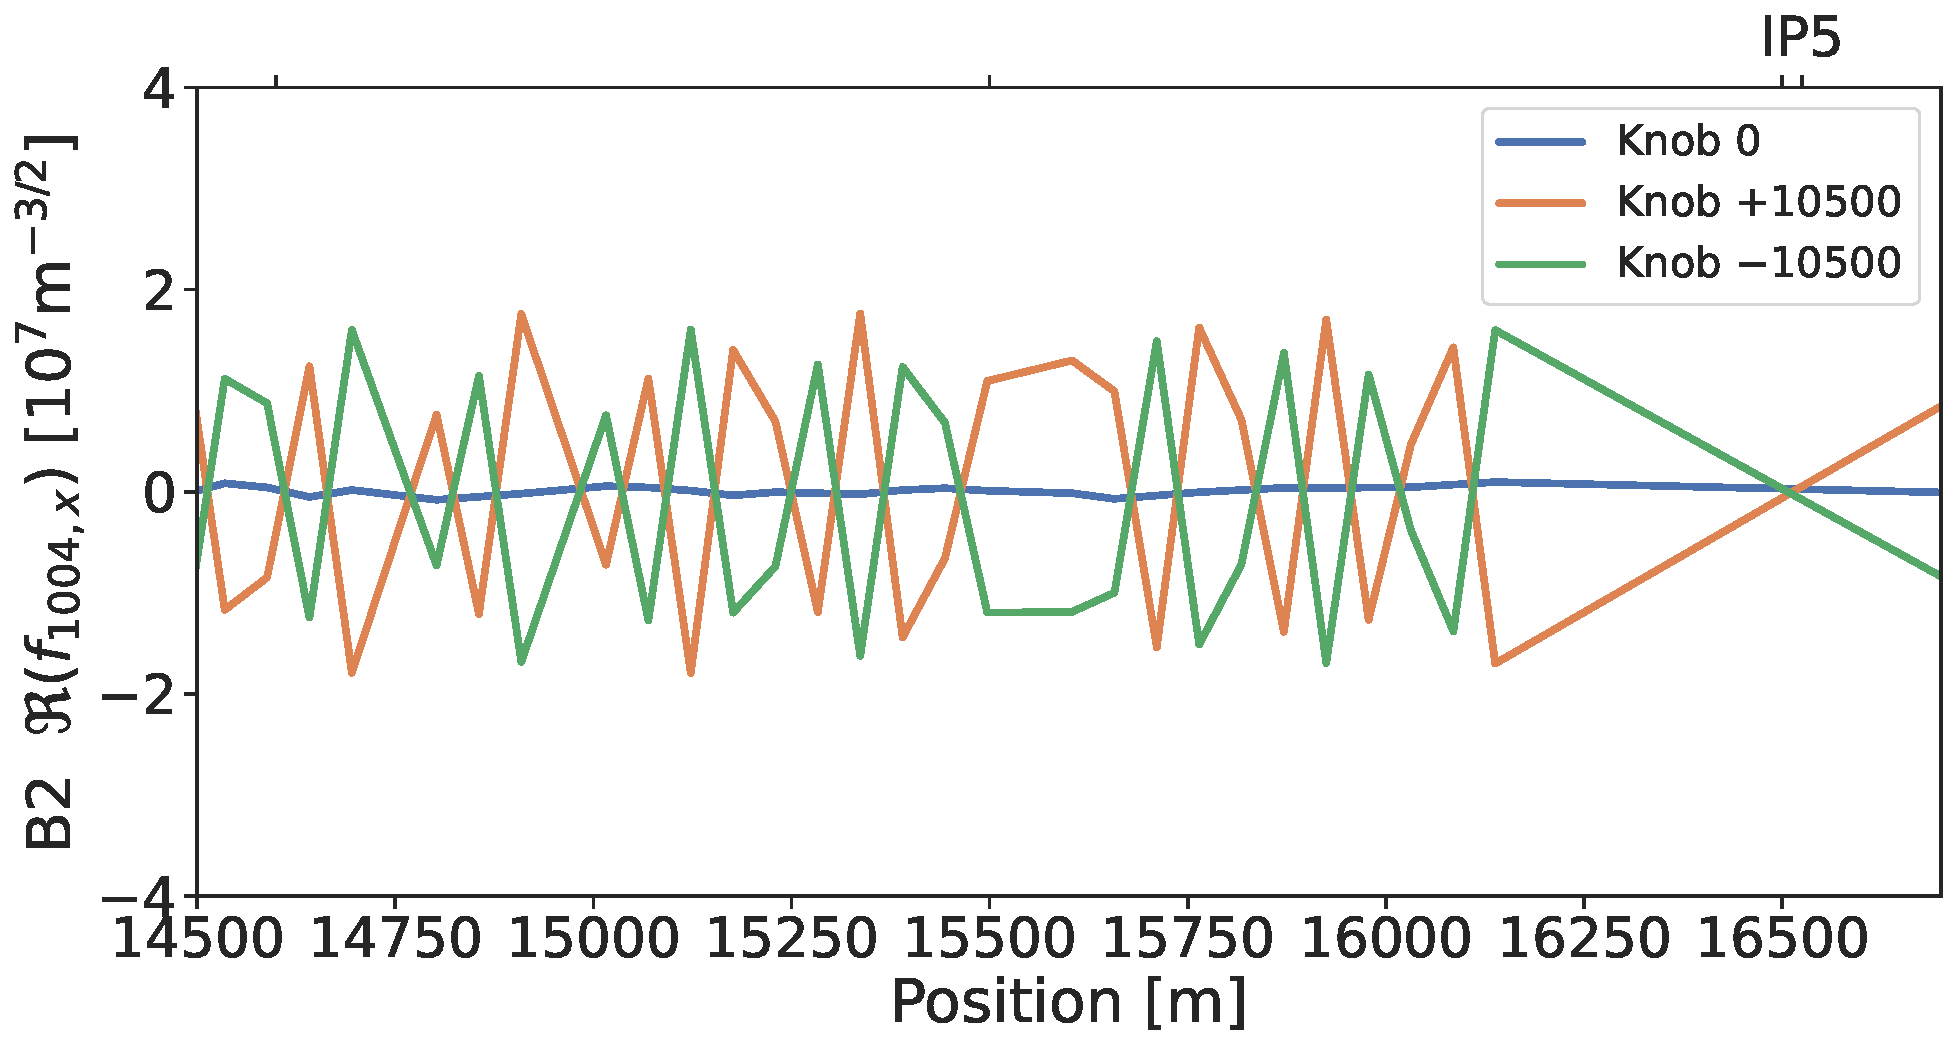
\includegraphics[width=0.8\textwidth]{./images/f1004/f1004x_knob_alt_lifetime_real.pdf}
    \caption{Measured real part of the RDT $f_{1004}$ depending on the powering scheme of the decapolar
    correctors.}
    \label{fig:decapoles:impact:alternating_knob}
\end{figure}

In order to measure the lifetime, a long period must be allocated as the signal returned from
monitors can be jittery. \cref{fig:decapoles:impact:b5_lifetime} shows this lifetime depending on
the decapolar strength scheme applied. The current of only one circuit is shown for readability.
A current of $\approx 230$ corresponds to a knob value of $+10500$ while a current of $-45$
corresponds to $0$.

\begin{figure}[!htb]
    \centering
    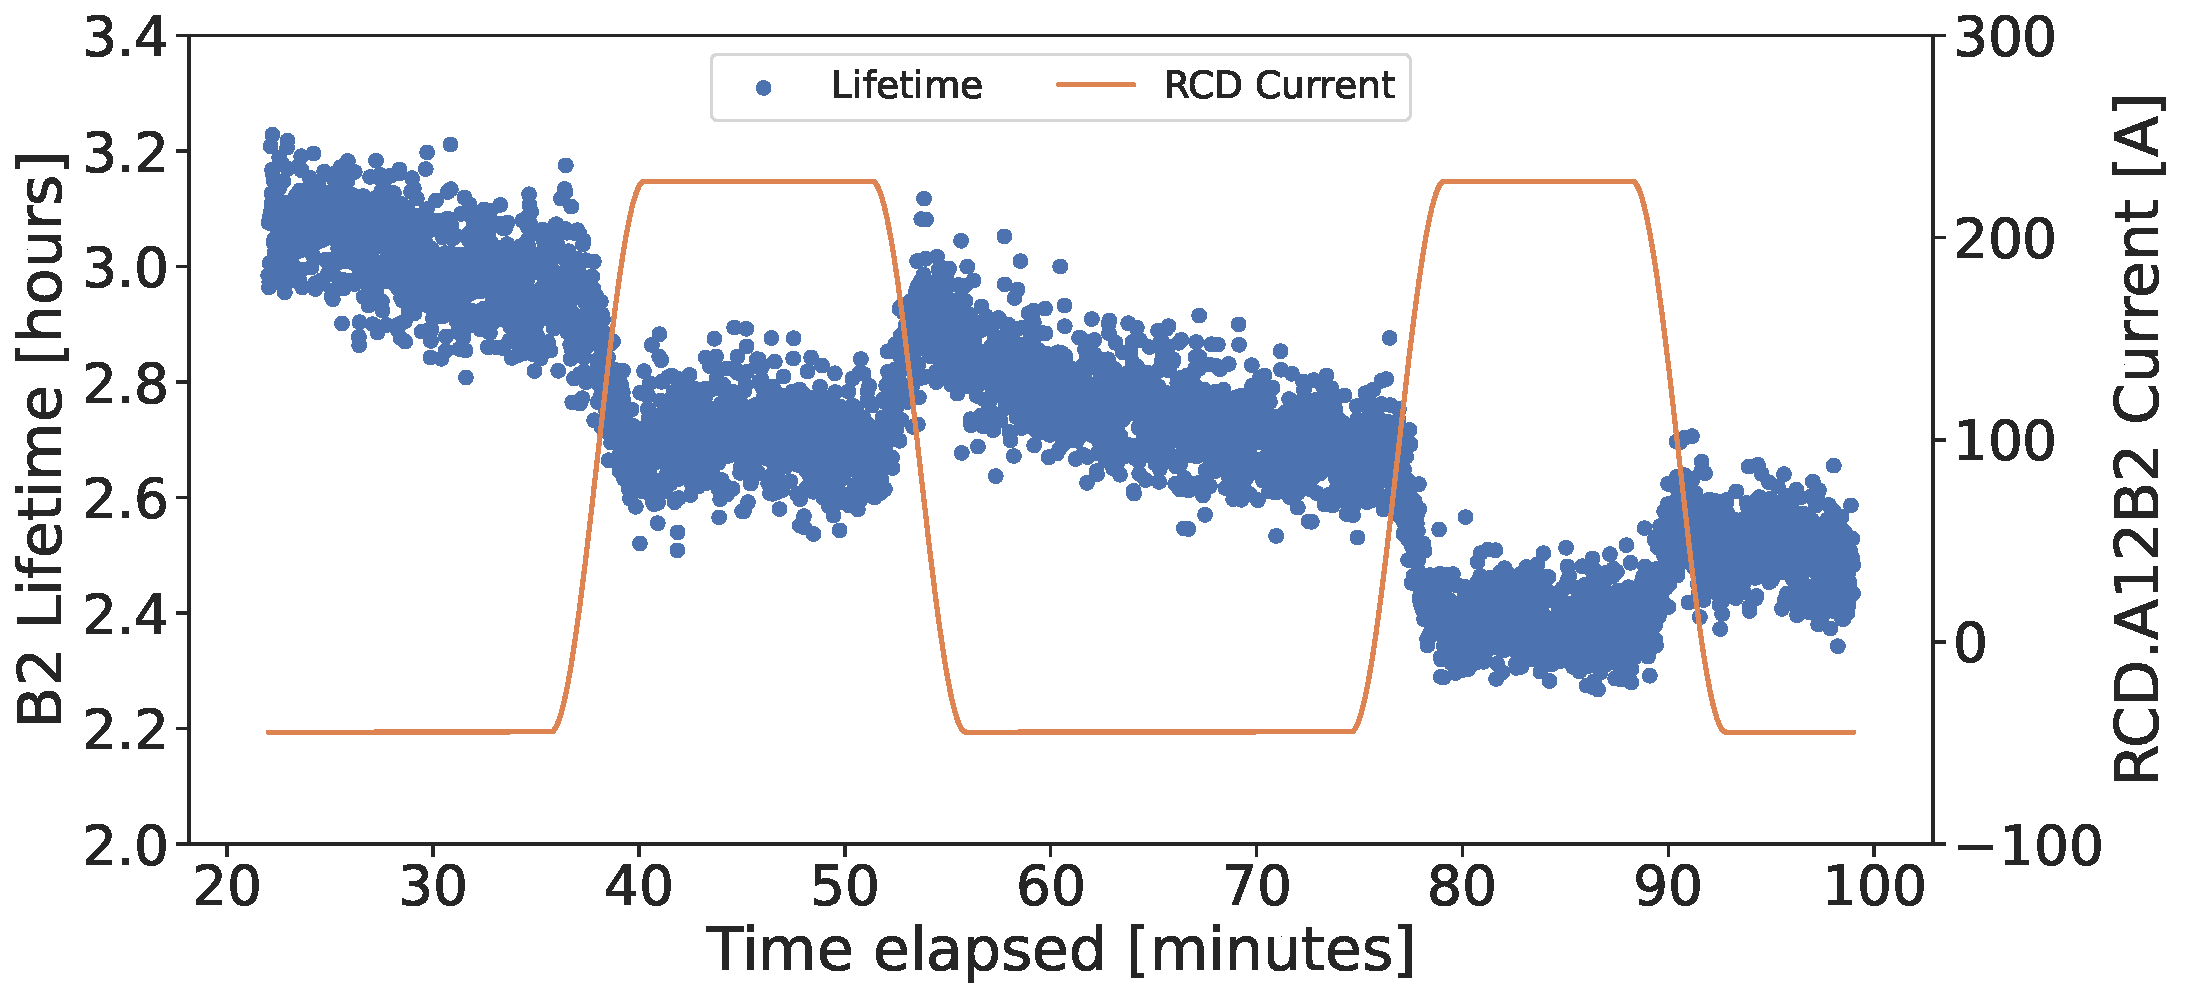
\includegraphics[width=0.8\textwidth]{./images/b5_lifetime.pdf}
    \caption{Measured lifetime of Beam 2 upon application of two different powering schemes for
    decapolar correctors. One trim keeps the RDT at a low amplitude while the other greatly
    amplifies it.}
    \label{fig:decapoles:impact:b5_lifetime}
\end{figure}

It is clear from this measurement that a large RDT decreases the lifetime of the beam.
The first pair of trim sees the average lifetime decreasing of $0.31 \pm 0.03$ hours, while the
second one sees a decrease of $0.36 \pm 0.03$ hours. This observed decrease of 20 minutes accounts
for $10\%$ of the beam lifetime at injection energy.


\paragraph{Corrections}

\todo{lifetime with f1004 and $Q'''$ corrections}

% 2023-06-14

% ---------------------------------------
%             subsection
% ---------------------------------------


